% !TEX encoding = UTF-8 Unicode
\documentclass[10pt,brazil]{beamer}
\usepackage[utf8]{inputenc}
\usepackage[brazil]{babel}
\usepackage{color,colortbl,multirow}
\usetheme{Luebeck}
\DeclareUnicodeCharacter{22EF}{ }
\usepackage{gensymb}
\setbeamertemplate{footline}
{
	\leavevmode%
	\hbox{%
		
		\begin{beamercolorbox}[wd=.666666\paperwidth,ht=2.25ex,dp=1ex,center]{title in head/foot}%
			\usebeamerfont{title in head/foot}\inserttitle
		\end{beamercolorbox}%
		\begin{beamercolorbox}[wd=.333333\paperwidth,ht=2.25ex,dp=1ex,right]{date in head/foot}%
			\usebeamerfont{date in head/foot}\insertshortdate{}\hspace*{2em}
			\insertframenumber{} / \inserttotalframenumber\hspace*{2ex} 
	\end{beamercolorbox}}%
	\vskip0pt%
}

\usepackage{caption}
\definecolor{azul}{HTML}{962038}
\setbeamercolor{structure}{fg=azul}
\usepackage{multicol}
\usepackage{media9}


\usepackage[alf]{abntex2cite}
\pgfdeclareimage[height=1.8cm]{logo}{UFOP}
\logo{\pgfuseimage{logo}}
\newcommand{\nologo}{\setbeamertemplate{logo}{}}
\setlength{\parskip}{0.2cm}

\title[Interface do Sistema de Arquivos]{Interface do Sistema de Arquivos}

\author[ICEA - UFOP]{Guilherme Marx, João Marcos, Bruno Passamai, Leonardo Sartori e Lucas Dau}

\begin{document}
 	   \maketitle
		\begin{frame}{Sumário}
			\tiny \tableofcontents
		\end{frame}
%---------------------------------------------------------


\section{Conceito de Arquivo}%11.1 - parte do possuído

\begin{frame}{Conceito de Arquivo}	
	
	\begin{itemize}

	\item Computadores armazenam informações através de diversos meios.
	\item Arquivo é uma coleção nomeada de informações relacionadas em armazenamento secundário.
	\item Arquivos podem ser:
	\begin{itemize}
		\item Numéricos;
		\item Alfabéticos ou
		\item Binários.
	\end{itemize}
	\item Possui certa estrutura definida que depende do seu tipo.
	\end{itemize}
\end{frame}

\subsection {Atributos de arquivo}
    
\begin{frame}{Atributos de arquivo}	
	\begin{itemize}

	\item Arquivos possuem atributos que variam de acordo com o Sistema Operacional. No geral são:
	\begin{itemize}
		\item Nome
		\item Identificador
		\item Tipo
		\item Local
		\item Tamanho
		\item Proteção
		\item etc
	\end{itemize}
	\item Essas informações são mantidas na estrutura do diretório.
	\end{itemize}
\end{frame}

\subsection{Operação de arquivo}
\begin{frame}{Operação de arquivo}    
	\begin{itemize}
	\item Um arquivo é um tipo abstrato de dado, logo, sobre ele são definidas algumas operações:
	\begin{itemize}
		\item Criação
		\item Escrita
		\item Leitura
		\item Busca
		\item Exclusão
		\item Truncamento
	\end{itemize}
	\item Outras operações comuns são acréscimo de informações ao final de um arquivo e renomeação. Essas operações primitivas podem ser combinadas para realizar outras operações como Cópia ou Recorte.
	\end{itemize}
	
	\end{frame}
      
\begin{frame}{Operação de arquivo}
	\begin{itemize}
	
	\item A maioria das operações envolvem pesquisa no diretório do arquivo.
	\item Muitos Sistemas Operacionais exigem o uso da Chamada de Sistema \emph{open()}. Dessa forma o Sistema Operacional mantém uma tabela contendo as informações dos arquivos abertos.
	\item Informações associadas a um arquivo aberto:
	\begin{itemize}
		\item Ponteiro de arquivo
		\item Contador de abertura de arquivo
		\item Local do arquivo no disco
		\item Direitos de acesso
	\end{itemize}
	\item Outro mecanismo oferecido pelos Sistemas Operacionais é o Locks de Arquivos.
	\end{itemize}  

\end{frame} 

\subsection{Tipos de arquivos}
\begin{frame}{Tipos de arquivos}
	
	\begin{itemize}
		
	\item Importantes para reconhecimento e aceitação de um arquivo.
	\item Uma técnica comum para implementá-lo é incluir o tipo como parte do nome.
	\end{itemize}   
	
	\begin{figure}[ht!]
		\centering
		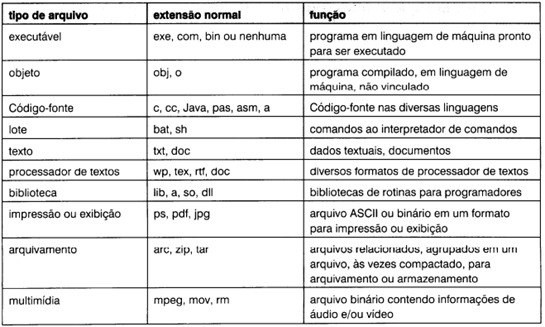
\includegraphics[scale=0.37]{tabela1.jpeg}
		\caption{Tipos de arquivos comuns}
		\label{Rotulo}
	\end{figure}
	
\end{frame}

\subsection{Estrutura do arquivo}
\begin{frame}{Estrutura do arquivo}
	\begin{itemize}
	
	\item Os tipos de arquivo também podem ser usados para indicar a estrutura de um arquivo.
	\item Arquivos de certos tipos devem corresponder às expectativas dos programas que os leem.
	\item Certos arquivos também precisam estar em conformidade com uma estrutura entendida pelo Sistema Operacional.
	\end{itemize}
\end{frame}

\subsection{Estrutura interna do arquivo}
\begin{frame}{Estrutura interna do arquivo}
	\begin{itemize}
	\item Localizar um deslocamento dentro de um arquivo pode ser uma tarefa complicada para o Sistema Operacional. 
	\item Toda a E/S de disco é realizada em unidades de um bloco e todos os blocos tem o mesmo tamanho.
	\item Uma solução para esse problema é empacotar registros lógicos em blocos físicos.
	\end{itemize} 
	
  \end{frame}
  
\section{Métodos de Acesso}%11.2 - parte do passamai
\begin{frame}{Métodos de Acesso}
	\begin{itemize}
	\item Arquivos armazenam informações que podem ser acessadas de duas formas:
		\begin{itemize}
		\item Acesso sequencial: Informações processadas em ordem, um registro após o outro.
		\item Acesso direto: Um arquivo com registros lógicos de tamanho fixo permite que programas leiam ou escrevam registros rapidamente sem qualquer ordem específica.
		\end{itemize}
	\item Outros métodos de acesso podem ser montados em cima de um método de acesso direto. Esses métodos em geral envolvem a construção de um Arquivo de índices.
	\item Para encontrar um registro, primeiro é pesquisado o índice e depois usamos o ponteiro para acessar o arquivo diretamente.
	\end{itemize}

\end{frame}  
  
  
\begin{frame}{Métodos de Acesso}
\begin{itemize}
\item Em arquivos muito grandes, o próprio arquivo de índices pode se tornar muito grande para ser mantido na memória. Uma solução é criar um índice para o arquivo de índice.
\item O arquivo de índice primário tem ponteiros para arquivos de índice secundários que apontam para os dados reais.
\item Para isso, podem ser utilizadas Árvores B ou variações.
\end{itemize}

\end{frame}
  
\section{Estrutura do diretório} %11.3 - parte do leo
\begin{frame}{Estrutura do diretório}
\begin{itemize}
\item Estruturas de diretório são utilizadas para organizar sistemas de arquivos muito grandes.
\item Essa organização é feita em duas partes. Primeiro os discos são divididos em uma ou mais partições.
\item Em segundo lugar, cada partição contém informações sobre os arquivos dentro dela. 
\end{itemize}
\end{frame}

\begin{frame}{Estrutura do diretório}
\begin{itemize}
\item Ao considerar uma estrutura de diretório, ela deve ser capaz de realizar algumas funções, tais como:
	\begin{itemize}
	\item Procurar um arquivo;
	\item Criar um arquivo;
	\item Excluir um arquivo;
	\item Listar um diretório;
	\item Renomear um arquivo;
	\item Atravessar o sistema de arquivos.
	\end{itemize}
\end{itemize}
\end{frame}

\begin{frame}{Estrutura do diretório}
\begin{itemize}
\item Esquemas mais comuns para definição da estrutura lógica de um diretório:
	\begin{itemize}
	\item Diretório de um único nível;
		\begin{itemize}
		\item Todos os arquivos contidos no mesmo diretório.
		\end{itemize}
	\item Diretório de dois níveis;
		\begin{itemize}
		\item Um diretório para cada usuário (UFD) e um diretório mestre (MFD) que aponta pro diretório do usuário.
		\item Arquivos do sistema são colocados em uma partição separada.
		\end{itemize}
	\item Diretórios estruturados em árvore;
		\begin{itemize}
		\item Permite aos usuários criarem seus próprios subdiretórios.
		\item Nome de caminho absoluto ou relativo.
		\end{itemize}
	\end{itemize}
\end{itemize}
\end{frame}

\begin{frame}{Estrutura do diretório}
\begin{itemize}
\item Esquemas mais comuns para definição da estrutura lógica de um diretório:
	\begin{itemize}
	\item Diretórios em grafo acíclico;
		\begin{itemize}
		\item A estrutura em grafo permite aos diretórios compartilharem subdiretórios e arquivos.
		\item Um arquivo pode possuir vários nomes de arquivo absoluto, como consequência, nomes de arquivos distintos podem se referir ao mesmo arquivo
		\end{itemize}
	\item Diretório geral do grafo.
	\begin{itemize}
	\item Mais eficiente que trabalhar com grafos acíclicos é garantir que não existem ciclos dentro de um grafo.
	\item Links e coleta de lixo.
	\end{itemize}
	\end{itemize}
\end{itemize}
\end{frame}


\section{Montagem do sistema de arquivos}%11.4 - parte do passamai
\begin{frame}{Montagem do sistema de arquivos}
\begin{itemize}
\item Um sistema de arquivos precisa ser montado antes de estar disponível para uso do Sistema Operacional.
\item Procedimento de montagem:
	\begin{enumerate}
	\item O Sistema Operacional recebe o nome do dispositivo e do ponto de montagem (local da estrutura de arquivos onde o sistema deve ser anexado).
	\item O SO verifica se o dispositivo contém um sistema de arquivos válidos
	\item O SO observa em sua estrutura de diretórios que o sistema de arquivos está montado no ponto especificado.
	\end{enumerate}
\item A partir daí, este já pode ser acessado pelo usuário.
\end{itemize}

\end{frame}

\section{Compartilhamento de arquivos}%11.5 - parte do Lucas
\begin{frame}{Compartilhamento de arquivos}
	\begin{itemize}
	\item Em um ambiente em que os arquivos são compartilhados por múltiplos usuários e múltiplos sistemas de arquivos estão presentes é esperado que dificuldades na coordenação do mesmo apareçam e o sistema operacional seja capaz de lidar com esses problemas.
	\end{itemize}
\end{frame}

\begin{frame}{Compartilhamento de arquivos}
\begin{itemize}
\item Dificuldades que podem ser observadas na coordenação de arquivos compartilhados:
	\begin{itemize}
	\item Múltiplos Usuários
	\item Sistemas de Arquivos Remotos
	\item Falhas
	\item Consistência
	\item Arquivos Imutáveis
	\end{itemize}
\end{itemize}
\end{frame}
\section{Segurança}%11.6 - parte do lucas

\begin{frame}{Segurança}
	\begin{itemize}
	\item A fim de manter a integridade dos arquivos, contra problemas do sistema, a estratégia é manter backups regulares para melhor proteção dos dados.
	\item Outra forma de proteger os dados de alterações feitas pelo usuário é o controle por tipo de acesso, como foi dito anteriormente. Assim o sistema é configurado para operações como leitura, escrita e exclusão. Podendo também ter controle por senha.
	\end{itemize}
\end{frame}

\section{Dúvidas}
\begin{frame}{Dúvidas}
\end{frame}
\section {Bibliografia}
\begin{frame}{Bibliografia}
\noindent[1] Silberschatz, A.; Galvin, P. B.; Gagne, G., Sistemas Operacionais com Java, Editora Campus, 7\textsuperscript{a} edição, 2008.
\newline

\noindent[2] Tanenbaum, A. S., Sistemas Operacionais Modernos, Editora Pearson, 3\textsuperscript{a} edição, 2010.
\newline

\noindent[3] Tanenbaum, A. S., Woodhull, A. S., Sistemas Operacionais: Projeto e Implementação. Editora Bookman, 3\textsuperscript{a} edição, 2008.
\end{frame}

\end{document}